\chapter{Monte-Carlo Tree Search}
\label{chap_mcts}

\todo{Add comment to Fig \ref{fig_mcts_loop}}
\begin{figure}
\begin{center}
\missingfigure{Obrázek ilustrující MCTS}
\end{center}
\caption{\footnotesize}{\footnotesize}
\label{fig_mcts_loop}
\end{figure}

\begin{algorithm}
\DontPrintSemicolon
\caption{$Select(tree)$\label{alg_select}}
\KwData{$tree$\ldots MCTS tree}
\KwResult{Leaf node chosen by the selection is returned. The selection is determined by a particular
$SelectionStep$.}
$curr\_node \leftarrow Root(tree)$\;
\While{$curr\_node \in T$}{
    $last\_node \leftarrow curr\_node$\;
    $curr\_node \leftarrow SelectionStep(curr\_node)$\;
}
\Return{$curr\_node$}\;
\end{algorithm}


\begin{algorithm}
\DontPrintSemicolon
\caption{$Backpropagate(tree, node, rewards[\,])$\label{alg_backpropagate}}
\KwData{$tree$ \ldots MCTS tree\\
$node$ \ldots node to which the rewards are being backpropagated\\
$rewards[\,]$ \ldots array of rewards }
\KwResult{$tree$ with playout rewards added to all $node$'s ascendants}
$AddRewards(node, rewards[\,])$\;
$parent \leftarrow Parent(node)$\;
\If{$parent \in tree$}{
    $Backpropagate(tree, parent, rewards[\,])$\;
}
\end{algorithm}

\todo{Komentář o tom, že může být odehráno více simulací ve fázi 3}
\todo{Komentář o možnosti využití výsledků z předchozích her}

\begin{algorithm}
\DontPrintSemicolon
\caption{$MCTSLoop(tree)$ \texttt{/* Main MCTS loop */}\label{alg_mcts}}
\KwData{$tree$\ldots MCTS tree}
\KwResult{$tree$ is enlarged by newly expanded nodes and results of playouts performed are added.
Node representing the best evaluated position reachable by one action is returned}
\While(\tcp*[h]{Main MCTS loop}){$EnoughTime()$}{
    $node \leftarrow Select(tree)$ \tcp*[h]{Phase 1: Selection}\;
    $node \leftarrow Expand(node)$ \tcp*[h]{Phase 2: Expansion}\;
    $rewards[\,] \leftarrow Playouts(node)$ \tcp*[h]{Phase 3: Simulation}\;
    $Backpropagate(tree,node,rewards[\,])$ \tcp*[h]{Ph 4: Backpropagation}\;
}
\Return{$\argmax\limits_{n \in Children(root)}c_n$} \tcp*[h]{Return most visited child}\;
\end{algorithm}

Monte-Carlo Tree Search (MCTS) is an iterative best-first search algorithm with stochastic positional
evaluation, anytime property and fast convergence. As \citeauthor{ChaslotPhd2010} summed up in 
\cite{ChaslotPhd2010}, MCTS was simultaneously developed
in three variants \cites{Chaslot2006}{Coulom2006}{Kocsis2006} in 2006. Specific variant used in
this thesis along with all important details and explanation of the properties is discussed in this
chapter. In addition, section \ref{sec_parallel_mcts} sumarizes current approaches to paralelization
of MCTS.

\section{Algorithm Description}

\citeauthor{Chaslot2008} provides good description of the Monte-Carlo Tree Search algorithm in
\cite{Chaslot2008}. Variant of MCTS as well as the terminology used in this thesis are based mainly
on this paper.

\todo{Je notace úplná?}
\todo{Sladit definice Perfect-information game s notací}

Monte-Carlo Tree Search is iteratively building the search tree as depicted by Figure
\ref{fig_mcts_loop} and Algorithms \ref{alg_select}, \ref{alg_backpropagate} and \ref{alg_mcts}
which follow the algorithm in its generality. Further details of chosen variant of MCTS
are discussed in subsequent sections and their related Algorithms, namely \ref{alg_selection_step},
\ref{alg_expand}, \ref{alg_playouts} and \ref{alg_add_rewards}.

Each node $i$ of the tree $t$ contains at least two values - visit count $n_i$
saying how many random position evaluations have been performed from $i$ and all its
descendants and
actual value $v_i$ which aggregates the results of these evaluations (usually as an average).
In addition, the game position represented by $i$, $Position(i)$, and pointers defining
tree structure have to be included. 

Position $p$ represents the current game state. Following
functions are appliable to $p$: $Actions(p)$ returns set of actions performable in $p$,
$Step(p, a)$ returns new position reachable by performing action $a$ in $p$ and $Score(p) \in
[0;1]$ returns static evaluation of the position (e.g. current game score).

$Parent(i)$ is
pointing to the parent of the node or to the $NullNode$ if $i$ is the root of the tree.
$Children(i)$ is the set of $i$'s children nodes. Once $i$ is expanded, $Children(i)$ contains
nodes representing positions reachable by set of
distinct actions $Actions(p)$ performable from $p = Position(i)$.
Particular action required to reaching $i$'s child $j$ is $Action(j)$.

New unexpanded node representing position $p$ reached with action $a$ is created by calling of
$new\;Node(p,a)$ where special $noop$ action is used for root node. Newly initialized tree for
planning from position $p$
containing only a root node is created with $new\;Tree(p)$.

The
tree itself provides the pointer to its root $Root(t)$. Function $EnoughTime()$ returns $true$ if
there is enough time to pass at least one more MCTS iteration and return the best evaluated node.

Each iteration of MCTS consists of four
phases - \emph{selection}, \emph{expansion}, \emph{simulation} and \emph{backpropagation}. During
the selection phase the 
algorithm passes through the tree to a particular leaf $i$ where better-evaluated but less-visited nodes
are preferred. Appropriate balance between these claims is main objective of this
phase. Once a leaf node is selected the expansion phase follows. In this phase, accordingly to a
certan condition (which is usually condition on node's visit count), $i$ itself is selected, or
new nodes reachable by actions from $Actions(i)$ are added to set $Children(i)$ and any of these
nodes is selected.
The next phase, simulation (also called \emph{playout}), plays a random game (or several games) 
starting
in position defined by expanded node halting on some conditions (e.g. after certain moves are
played or the end of the game is reached). Results from the simulations are then backpropagated to all
expanded node's ancestors during the fourth phase - backpropagation. The phases of the algorithm are
further discussed in subsequent sections.



\subsection{Selection}

\begin{algorithm}
\DontPrintSemicolon
\caption{$SelectionStep(node)$\label{alg_selection_step}}
\KwData{$node$\ldots a node of MCTS tree}
\KwResult{a children node chosen by a selection}
\If(\tcp*[h]{$node$ is a leaf or terminal node}){$Children(node)=\varnothing$}{
    \Return{$NullNode$}
}
\If(\tcp*[h]{Not enough simulations played}){$n_{node} < T_s$}{
    \Return{$SimulationStep(node)$} \tcp*[h]{Follow simulation strategy}
}
\If{$\exists i \in Children(node)$ such that $n_i=0$}{
    \Return{$i$} \tcp*[h]{Try all children first}
}
\Return{$\argmax\limits_{i \in Children(node)} \left( v_i + C \sqrt{\log{n_{node}} \over n_i}
\right)$} \tcp*[h]{Follow UCT value}
\end{algorithm}

The process of selection consists of selection steps passing from a node to one of its children.
Each such a step meets exploration-exploitation problem where exploitation tends to choose the
so far best evaluated node and exploration on the other side promotes
undiscovered ways in the tree. This problem can be viewed as instance of a well-known problem 
called the Multi-Armed Bandit Problem (MAB). Its definition is adopted from \cite{Auer2002} and 
\cite{Kocsis2006}:

\newtheorem*{defmab}{Definition}
\begin{defmab}[K-armed bandit problem] 

Let us have independent random variables $X_{i,n}$ for $1 \le i \le K$ and $n \ge 1$. Each $i$ is
the index of a gambling machine and $X_{i,1}$, $X_{i,2}$,\ldots are identically distributed rewards
with unknown expected value $\mu_i$ yielded by successive plays of machine $i$. For the simplicity
the rewards are bounded to $[0,1]$.

A \textbf{policy} $A$ is an algorithm that chooses the next machine to play based on the sequence of
past plays and obtained rewards. Let $n_i$ be the number of times machine $i$ has been played by
$A$ during the first $n$ plays and $I_i^A$ be the index of a machine played in nth play. Then the
regret of A after n plays is defined as

\begin{equation}
R_n^A = n \mu^* - \sum_{j=1}^K n_j \mu_j \mathrm{,\;where}\;\mu^* \stackrel{\mathrm{def}}{=}
\max_{1 \le i \le K} \mu_i
\end{equation}

thus the \textbf{regret} $R_n^A$ is the loss caused by the policy not always playing the best machine.

\textbf{K-armed bandit problem} consists in finding optimal policy $A^*$ minimizing
expected regret $R_n^A$.

\end{defmab}

\todo{Citovat \cite{Berry85banditproblems}}
\todo{doplnit zmínku o tom, že optimální policy má regret  ~$O(\log{n})$,
ale že je výpočetně náročná}

\Citeauthor{Auer2002} introduced computationaly effective optimal policy UCB1 \cite{Auer2002} 
having regret bounded to $O(\log{n})$. Abbreviation UCB stands for \emph{Upper-Confidence Bound}
and refers to value maximized by the policy. Let us define the value of UCB1:

\begin{equation}
UCB1(\bar{X}_{i,n_i},n,n_i) = 
    \left\{
        \begin{array}{c@{\quad\quad}l}
            \bar{X}_{i,n_i} + \sqrt{{2 \log{n}} \over n_i} & if \quad n_i > 0 \\
            \infty & otherwise \\
        \end{array}
    \right.
\end{equation}.


Then the policy itself chooses the machine as follows:

\begin{equation}
 I_{UCB1}(n+1) = \argmax\limits_{i\in{1,\ldots,K}} UCB1(\bar{X}_{i,n_i},n,n_i)
 \end{equation}.

UCB1 consists of average of previous rewards and a bias decreasing with number of the
machine's plays. In addition significance of the bias is growing with the total number of plays
which 
leads to increase of exploration. Each machine is tried once before further selection based on
previous evaluation and the bias is used. This is forced by setting UCB1 value to $\infty$ for
machines not yet tried.

UCB1 applied to Trees \cite{Kocsis2006} is derived from UCB1 using values $v_i$ and $n_i$ stored in
particular node $i$. In addition the bias coefficient C is introduced in \cite{Chaslot2008}.
The purpose of this coefficient is tuning the balance between exploration and exploitation.
UCB1 contains fixed value of $C$ equal to $\sqrt{2}$ which can be used as good reference value.
Tuning of $C$ is usually done 
experimentally. The form of the formula for UCT and related selection applied in node $p$ is as
follows:

\begin{align}
    &\begin{aligned}
UCT(v_i,n_p,n_i) &= \left\{
        \begin{array}{c@{\quad\quad}l}
            v_i + C \sqrt{{\log{n_p}} \over n_i} & if \quad n_i > 0 \\
            \infty & otherwise \\
        \end{array}
    \right.
    \end{aligned}\\
    &\begin{aligned}
I_{UCT}^p &= \argmax\limits_{i \in Children(j)} UCT(v_i, n_p, n_i)
    \end{aligned}
\end{align}



Accordingly to the UCT, the selection passes down through the tree starting in the
root where the child with greatest UCT value is chosen in each node until a leaf is reached.
As mentioned in \cite{Chaslot2008}, experimental results show that the UCT value does not 
guide the selection well until
enough trials have been performed in node $p$ ($n_p$ is too small). To overcome this empirical
finding, the selection is guided by \emph{simulation strategy} which uses domain-specific
information (described in section
\ref{sec_simulation}) until $n_p$ does not reach certain threshold T. Selection phase
consisting of selection steps is
depicted by Algorithm \ref{alg_select}. The selection steps is then depicted by Algorithm
\ref{alg_selection_step}. In MCTS for a game of Go in \cite{Chaslot2008} the constants used
are $C= 0.7$ and $T=30$.




\subsection{Expansion}
\label{sec_expansion}

\todo{Popsat v textu notaci new Node() a new Tree()}

\begin{algorithm}
\DontPrintSemicolon
\caption{$Expand(node)$\label{alg_expand}}
\KwData{$node$\ldots a leaf node of MCTS tree}
\KwResult{$node$ itself is returned, or new children reachable by actions valid in position
defined by $node$ are added to
$node$. One if these children is then returned.}
\If(\tcp*[h]{Not enough simulations performed}){$n_{node} < T_e$}{
    \Return{$node$}
}
\If(\tcp*[h]{$node$ is a terminal node}){$Actions(node) = \varnothing$}{
    \Return{$node$}
}
\ForEach{$action \in Actions(node)$}{
    $next\_pos \leftarrow Step(Position(node), action)$\;
    $child \leftarrow new\;Node(next\_pos, action)$\;
    $Children(node) \leftarrow Children(node) \cup \{ child \}$\;
}
\Return{$child$}
\end{algorithm}

The expansion decides whether or not will be the selected leaf expanded and so if the simulation
will begin in the leaf itself or in one of its children. The most common variant used also in our
thesis is that the node is
expanded once it reaches a particular visit count $T_e$. Greater value in such a condition causes higher
simulation count in each node and so stronger evaluation. On the other hand the process of building
tree is slowed down. With $T_e=1$ the expansion becomes even simplier and the leaf is simply
expanded always. Algorithm \ref{alg_expand} ilustrates expansion performed after $T_e$
simulations have been performed from a leaf.


\subsection{Simulation}
\label{sec_simulation}

\begin{algorithm}
\DontPrintSemicolon
\caption{$Playouts(node)$\label{alg_playouts}}
\KwData{$node$\ldots a node of MCTS tree}
\KwResult{An array of results of performed simulations is returned.}
\For{$i\leftarrow 1$ \KwTo $SIMULATIONS\_COUNT$}{
    $p \leftarrow Position(node)$\;
    \While{$\mathbf{not}\;TerminalCondition(p)$}{
        $p \leftarrow Step(p, SimulationAction(p))$\;
    }
    $rewards[i] \leftarrow Score(p)$\;
}
\Return{$rewards[\,]$}
\end{algorithm}

The simulation, or \emph{playout}, performs random play starting in the position defined in the
node selected by previous phases - selection and expansion. Simulation steps can be plain
random moves or, to improve the strength of
simulation, the simulation can follow a pseudo-random \emph{simulation strategy} designed accordingly to
domain-specific information. The stochasticity of chosen simulation strategy determines the strength
of simulation. If the strategy is too stochastic, or on the contrary too deterministic, the
simulation strenght is decreasing and it is difficult to choose adequate compromise.

Simulation is terminated if a certain condition is encountered (e.g. limit on number of simulation
steps or the end of the round is reached) and player's position score from interval $[0;1]$ is
returned. Additionally, to speed up the simulation the simulation steps can be performed in
simplified game environment.

Even if it is better to perform selection before each simulation to avoid multiple 
evaluations of weak positions, some cases requires running multiple simulations in this phase
(e.g. \emph{leaf parallelization} described in section \ref{sec_leaf_parallelization}). This is
the reason why the array of results is returned by $Playouts(node)$ depicted by Algorithm
\ref{alg_playouts} Number of simulations performed is denoted as $SIMULATIONS\_COUNT$, action
selected by simulation strategy in position $p$ as $SimulationAction(p)$ and terminal condition
as $TerminalCondition(p)$.


\subsection{Backpropagation}

The last phase of the MCTS iteration is the backpropagation. The task of this phase is to propagate
rewards provided by the simulation to all node's precedessors. Various backpropagation strategies
may be used, however, the plain average is crucial for good properties of UCT and performs
well in
practise. Hence the result set $rewards[\,]$ obtained by simulation is added to the node's value containing
average of simulations performed in its subtree which leads to the update formulae for
node $p$ used in Algorithm \ref{alg_add_rewards}.

\begin{algorithm}
\DontPrintSemicolon
\caption{$AddRewards(node,rewards[\,])$\label{alg_add_rewards}}
\KwData{$node$\ldots a node of MCTS tree\\$rewards[\,]$\ldots array of simulation rewards}
\KwResult{Simulation results $rewards[\,]$ are added to $node$'s value.}
$rlen \leftarrow Length(rewards[\,])$\;
$rsum \leftarrow \sum\limits_{i=1}^{rlen} rewards[i]$\;
$v_{node} \leftarrow {{v_{node} n_{node} + rsum}
    \over{n_{node} + rlen}}$\;
$n_{node} \leftarrow n_{node} + rlen$\;
\end{algorithm}



\section{Convergence to Minimax algorithm}
\label{sec_minimax_convergence}



\section{MCTS for Two-Player Games}
\label{sec_two_players_mcts}
\emph{Discussion about simultaneous v. turn-based games and its convergence}

However it has been shown that MCTS converges to... \emph{TODO: Načíst jak je to s konvergencí k
minimax stromu a pure nash equilibrium strategii a opravit podle toho předchozí text}. Odkázat se
na \ref{sec_turn_based_game_conversion}.


\section{Parallel Monte-Carlo Tree Search}
\label{sec_parallel_mcts}

\todo{Zvážit změnu terminologie (multi-core, cluster, thread, core)}

Our objective in this thesis is designing algorithms for distributed MCTS computation among
cooperating agents. Closest to such algorithms are works on parallelization of MCTS which are
strong inspiration for algorithms proposed in chapter \ref{chap_dmcts_design}.

Several publications dealing with parallelization of Monte-Carlo Tree Search have been published
recently \cites{Cazenave2007}{Chaslot2008}{Teytaud2008}. Two kinds of the parallelization are
discussed in these papers - multi-core parallelization and cluster parallelization.

Multi-core parallelization refers to computation on a symmetric multiprocessor computer (SMP). In
this case memory is shared among all processor cores and and can be accessed with same
(generally low) latency by any core  and access to this memory is the same and low.
Access synchronization have to be managed using a mutex mechanism. Two techniques for
parallelization with no need for locking (\emph{leaf parallelization}, \emph{root parallelization},
\emph{simulation results passing}),
and two variants of parallelization with locking (\emph{tree parallelization}) have been proposed so
far. 

Cluster parallelization is more generalized approach to parallelization. Memory is not shared
between parallel processes and so the inter-process communication is realized by \emph{message
passing}. Latencies in inter-process communication have to be taken in consideration but on the
other hand no memory locking is necessary. Algorithms mentioned as not using memory locking in
previous paragraph are suitable also for cluster parallelization.

For the simplicity and due to fact that all algorithms can be used in multi-core environment, we 
use multi-core terminology in descriptions of algorithms, so parallel
computational flows will be referred as \emph{threads} and computational nodes as \emph{cores}.

Strength and speed measures for comparing of algorithms used in this section is described in
following section.

\subsection{Comparison Measures for Parallel MCTS Algorithms}
\label{sec_measures_parallel}

We will briefly describe measures used in comparisons of parallel MCTS algorithms described in
following sections. Measures are derived from \cite{Chaslot2008}.

\emph{Strength} of a player choosing actions for playing a game $G$ against
opponents $O$ (for case of multi-player game) \todo{Tady by se dalo napsat víc o tom, jak volit
oponenty}
is expected value of player's score at the end of the game. For experimental evaluation of the
strength, finite set of games is played and average
\todo{std dev?}
 of scores obtained is used. For our
purposes the player is guided by MCTS-based algorithm. Its strength is dependent on time $T$
provided to the algorithm for computation. In case of parallel MCTS algorithms, each thread has
time $T$ for computation. Since parallel algorithms run in multiple threads, each having same
amount of time as plain MCTS, its strength should be greater than in case of plain MCTS and should 
grow with number of cores $n$ involved. For more ilustrative comparison of parallel algorithms,
we will use \emph{strength-speedup} measure. Let us consider parallel algorithm having time
$T_{par}$
for its running and its strength $S$. Plain MCTS needs time $T_{pl}$ to achieve same strength
$S$. Then strength-speedup is equal to ratio of $T_{pl} \over T_{par}$. In other words,
strength-speedup is the increase of time needed to achieve the same strength by plain MCTS.
For better comparison of parallel algorithms running on various numbers of threads, we will use 
the third measure, a ratio of strength-speedup to the number of cores available for parallel
algorithm, and call it \emph{strength-efficiency}. This ratio can be also seen as ratio between
resources needed by plain MCTS (only $T$) and parallel MCTS ($T$ multiplied by number of
cores).

Another measure appliable to MCTS is \emph{Simulations-per-Second}. It simply says how many
simulations per second is being performed. Analogically to strength measures,
\emph{Simulations-per-Second speedup} and \emph{Simulations-per-Second efficiency} are defined
as ratio of Simulations-per-Second of plain MCTS and parallel MCTS and same ratio divided by
number of cores. These measures are very useful for comparison of effectiveness of
parallelization and so we will refer to Simulations-per-Second speedup simply as
\emph{speedup}. \todo{Doplnit tabulku s mírami}





\subsection{Leaf Parallelization}
\label{sec_leaf_parallelization}

\begin{algorithm}
\DontPrintSemicolon
\caption{$LeafParallelizationPlayouts(node)$}
\label{alg_leaf_parallelization}
\KwData{$node$\ldots a node of MCTS tree}
\KwResult{Array of simulation resulults is returned}

$tree \leftarrow new\,McTree$ \tcp*[h]{Initialize empty tree}\;
$root \leftarrow Root(tree)$\;
\ForEach{available processor core $C$}{
    $thread\_count \leftarrow thread\_count + 1$\;
    $threads[thread\_count] \leftarrow new\,PlayoutThread$\;
    $Run(thread)$\;
}
\While(wait for simulations){$AnyThreadRunning(threads)$}{
    $Wait()$\;
}
\For{$i\leftarrow 1$ \KwTo $Length(threads[\,]$}{
    $rewards[i] \leftarrow Reward(threads[i])$\;
}
\Return{$rewards[\,]$}
\end{algorithm}

\emph{Leaf parallelization} is simple algorithm originally introduced in \cite{Cazenave2007} as
\emph{at-the-leaves parallelization}. Parallelization is used only during simulation phase where
multiple simulations are executed. 

Master thread traverses the root to the leaf according to selection strategy and expands selected
leaf at first. Then for each available processor core, one simulation is performed from position
defined by leaf. Master thread then waits until all simulations are finished and backpropagates
their results up through tree. Algorithm \ref{alg_leaf_parallelization} depicts simulation phase 
of leaf parallelization. \todo{Popis metod v algoritmu (ThreadSet etc..)}

This approach is very easy to implement since no complicated synchronization is used
which is its main advantage. However, several disadvantages have to be mentioned. First, cores are
not fully loaded for two obvious reasons. Algorithm is single-threaded during selection, expansion
and backpropagation phases and so slave threads are sleeping. In addition, running time of
simulation threads differ due to their high unpredictability and threads which already finished
simulation have to wait for the last one. Second disadvantage is one that leaf parallelization
forces multiple simulations
per position. It leads to better position evaluation but slows the speed of tree building. Last
disadvantage is that in comparison with plain MCTS which performs selection after each simulation,
the leaf parallelization have to perform full set of simulations per each node and so some of
unnecessary simulations are uselessly performed because first few of them can serve as good evidence
for considering the position as a bad candidate for further exploration. This can be worked around
if simulation threads are terminated once such a consideration is made according to already finished
simulations.

Leaf parallelization is suitable for using in both multi-core and cluster environment.


\subsection{Root Parallelization}
\label{sec_root_parallelization}

\begin{algorithm}
\DontPrintSemicolon
\caption{$RootParallelizationMaster(random\_seed)$}
\label{alg_root_parallelization_master}
\KwData{$random\_seed$\ldots a random seed distincts from seeds of other threads}
\KwResult{Best move calculated by root parallelization alrogithm}

$tree \leftarrow new\,McTree$ \tcp*[h]{Initialize empty tree}\;
$MCTSLoop(tree)$ \tcp*[h]{Perform MCTS iterations}\;
$roots \leftarrow new\,RootSet$ \tcp*[h]{Empty set}\;
$roots \leftarrow roots \cup BuildNextActionTreeCut(tree)$ \tcp*[h]{Add own root}\;

\ForEach(\tcp*[h]{Receive roots}){Team-mate $P$}{
    $received\_root \leftarrow Receive(P)$\tcp*[h]{Wait for a root from $P$} \;
    $roots \leftarrow roots \cup received\_root$\;
}

\tcp*[h]{Merge roots} \;
$merged \leftarrow new\,McTree$ \;
\ForEach{$root \in roots$}{
    \ForEach{$leaf \in Leaves(root)$}{
        $node \leftarrow LookupNode(merged,Path(leaf))$ \tcp*[h]{new node is created if not found}\;
        $Backpropagate(merged,node,RewardsOf(leaf)$ \tcp*[h]{$leaf$ is merged into the tree} \;
    }
}

\Return{$\argmax\limits_{n \in Children(Root(merged))}c_n$} \tcp*[h]{Return most visited child}\;
\end{algorithm}

\begin{algorithm}
\DontPrintSemicolon
\caption{$RootParallelizationSlave(random\_seed,master\_thread)$}
\label{alg_root_parallelization_slave}
\KwData{$random\_seed$\ldots a random seed distincts from seeds of other threads\\
$master\_thread$\ldots master thread}
\KwResult{Nothing. Best move is returned by master thread.}
$tree \leftarrow new\,McTree$ \tcp*[h]{Initialize empty tree}\;
$MCTSLoop(tree)$ \tcp*[h]{Perform MCTS iterations}\;
$root \leftarrow BuildNextActionTreeCut(tree)$ \tcp*[h]{Extract root}\;
$Send(master\_thread, Message(root))$\;
\end{algorithm}

Another approach first proposed in \cite{Cazenave2007} is \emph{root parallelization} being
originally named as \emph{single-run parallelization}. In root parallelization, independent
MCTS instance is executed for each core with different random-seeds so the trees built by individual
instances differ. Finally, roots with their children from all instances are collected in master
thread and merged. The result is set of nodes containing information from all MCTS instances which
are used for selecting the best action to perform. Main advantages are simple implementation and a
minimal amount of communication so root parallelization can be successfully used both in cluster
and multi-core environment.

The algorithm is ilustrated by Algorithms \ref{alg_root_parallelization_master} and 
\ref{alg_root_parallelization_slave} (1 master together with several slaves are run). 
In the algorithm, we use 
procedure $BuildNextActionTreeCut$ for extraction of tree root. Description of the procedure
and related pseudocode can be found in Section \ref{sec_root_exchanging_agents}.

There is a disadvantage resulting from missing communication during running of MCTS
instances. Because each MCTS tree is built separately each instance have to perform similar
exploration or in other words same set of positions have to be evaluated before interesting
positions can be inspected. Due to this disadvantage plain MCTS having proportionally more time for
running would still probably perform better because no duplicit exploration have to be done and such
a saved time can be used for deeper exploitation. However, accordingly to comparisons resumed
in Section \ref{sec_parallel_mcts_comparison}, the root parallelization performs, at least for the 
game of Go, approximately equally to plain MCTS having adequately more time for computations
(time used by root parallelization algorithm times number of processors used).

\subsection{Tree Parallelization}

\todo{pseudocode}

The reasons why leaf parallelization wastes too much time leaving cores in sleep are removed by
\emph{tree parallelization}. It is done by effective tree locking so individual threads can access
and modify the tree on their own and so particular simulations follow independent selections and
need not to wait for the end of other simulations. The tree can be locked with \emph{global mutex}
or with \emph{local mutexes} placed all nodes. The global mutex is simplier method saving costs
associated with locking but the maximum speedup is significantly reduced because the average
percentage of time spent in the tree (denoted as $x$ for now) is relatively high ($25\%-50\%$) and
so it is not possible to reach speedup higher than $100/x$. This is because if each of $n$
threads is
accessing the tree exclusively and no one have to sleep, percentage of time spent in 
tree is
equal to $n x$ and so $n \le \lfloor {100 \over{x}} \rfloor$. Due to this limitation, local mutexes
are necessary for systems with greater number of cores. To beat the fact of high cost of locking and
unlocking, fast-access mutexes should be used (i.e. spinlocks).

One more disadvantage of leaf parallelization should be handled which is parallel evaluation of a
single node when multiple evaluations are performed even if the first one may mark the node badly
and so not recomment for further exploitation. To prevent additional evaluations before previous
ones are currently running \emph{virtual loss} is added to the value of the node being evaluated
and remove it then during backpropagation.
If the virtual loss is chosen properly, further evaluations are performed only in case when the
node's value is good enough even after adding the virtual loss and so weak nodes are not paralelly
evaluated.



\subsection{Simulation Results Passing}
\label{sec_simulation_passing}

\begin{algorithm}
\DontPrintSemicolon
\caption{$SimulationResultsPassingLoop(tree)$}
\label{alg_simulation_results_passing}
\KwData{$tree$ \ldots MCTS tree}
\KwResult{$tree$ is enlarged by calculated and received simulations}

\While(\tcp*[h]{Main MCTS loop}){$EnoughTime()$}{
    \While(\tcp*[h]{Receive messages}){Receiving queue $Q$ not empty}{
        $(path,rewards[\,]) \leftarrow Pop(Q)$ \;
        $node \leftarrow LookupNode(tree,path)$ \tcp*[h]{new node is created if not found}\;
        $Backpropagate(tree,node,rewards)$ \;
    }
    $node \leftarrow Select(tree)$\;
    $node \leftarrow Expand(node)$\;
    $rewards[\,] \leftarrow Playouts(node)$\;
    $Backpropagate(tree,node,rewards[\,])$ \;
    \ForEach(\tcp*[h]{Send messages}){Team-mate $P$}{
        $SendSimulationResult(P, Message(Path(node),rewards[\,]))$ \;
    }
}

\Return{$\argmax\limits_{n \in Children(root)}c_n$} \tcp*[h]{Return most visited child}\;
\end{algorithm}



\emph{Simulation results passing} can be viewed as a trial of adaptation of \emph{tree
parallelization} to cluster environment. These two algorithms share the property of high amount of
communication which is naturally bigger problem in distributed environment.

Unlike tree parallelization, the simulation results passing is building search tree separately in
each thread and synchronizes these trees by broadcasting messages containing identification of
expanded node and resulting value of performed simulation. This value is then backpropagated in
trees of receiving threads. Master thread finally returns best move accordingly to its tree.
Simulation results passing is depicted by Algorithm \ref{alg_simulation_results_passing}.

This algorithm relies on high throughput of the cluster environment. Requirements on the throughput
grows with number of parallel threads so algorithm is not suitable for massive parallelism. The
algorithm is designed for usage in cluster environment but can be of course used also in multi-core
environment.


\subsection{Comparison and Conclusion}
\label{sec_parallel_mcts_comparison}

We have sumarized known algorithms for parallelization of MCTS in both multi-core and cluster
environment. Three of them (leaf parallelization, root parallelization and tree
parallelization)
have been experimentally evaluated in \cite{Chaslot2008} in context of playing Go in multi-core
environment. For this purpose the \emph{strength speedup} measure has been used. It is equal to
 the ratio of time needed for plain
MCTS to reach the same strength. Brief summary of results is covered by Table
\ref{tab_parallel_mcts_comparison} and Figure \ref{fig_parallel_mcts_comparison}. The winner of comparison is root parallelization performing even
better than single-threaded MCTS in case of 2 and 4 parallel threads. This is interpreted as 
parallel MCTS algorithms with different random seeds exploit different local optima so better one
can be finally chosen. Second best performance showed tree parallelization using virtual loss. Other
algorithms performed very poorly especially in case of higher number of threads.

\begin{figure}
\begin{center}
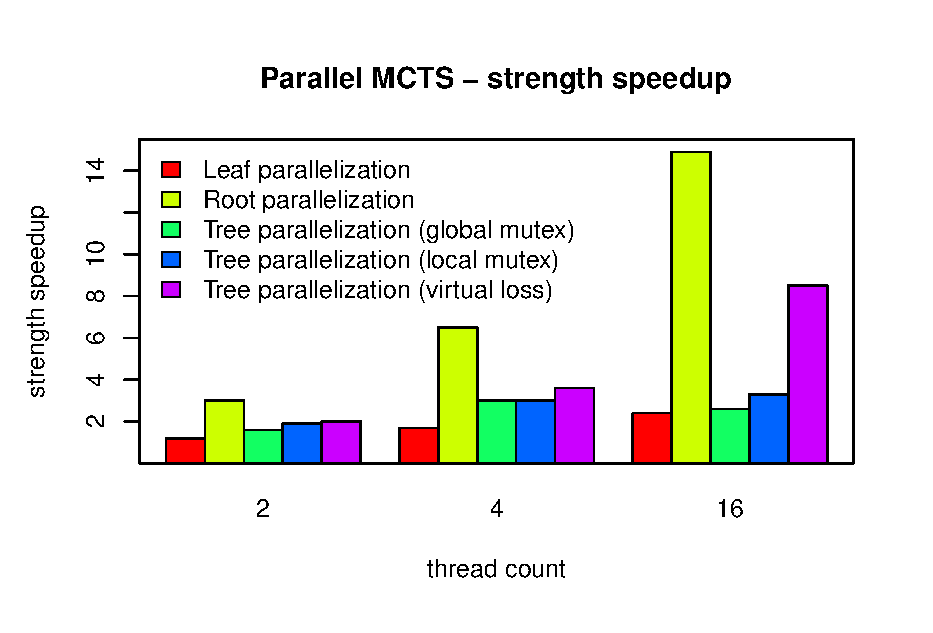
\includegraphics{img/parallel-mcts.eps}
\end{center}
\caption{\footnotesize Lorem ipsum}{\footnotesize }
\label{fig_parallel_mcts_comparison}
\end{figure}

\begin{table}[h]
\begin{center}
\begin{tabular}{|l|rrr|}
\hline Algorithm & 2 threads & 4 threads & 16 threads\\
\hline Leaf parallelization & 1.2 & 1.7 & 2.4\\
\hline Root parallelization & 3.0 & 6.5 & 14.9\\
\hline Tree parallelization (global mutex) & 1.6 & 3.0 & 2.6\\
\hline Tree parallelization (local mutex) & 1.9 & 3.0 & 3.3\\
\hline Tree parallelization (virtual loss) & 2.0 & 3.6 & 8.5\\
\hline
\end{tabular}
\end{center}
\end{table}

%\begin{table}[h]
%\begin{center}
%\begin{tabular}{lrr}
%\hline
%Algorithm & Thread count & Strength speedup\\
%\hline
%Leaf parallelization & 2  & 1.2\\
%Leaf parallelization & 4  & 1.7\\
%Leaf parallelization & 16 & 2.4\\
%\hline
%Root parallelization & 2  & 3.0\\
%Root parallelization & 4  & 6.5\\
%Root parallelization & 16 & 14.9\\
%\hline
%Tree parallelization (global mutex) & 2  & 1.6\\
%Tree parallelization (global mutex) & 4  & 3.0\\
%Tree parallelization (global mutex) & 16 & 2.6\\
%\hline
%Tree parallelization (local mutex) & 2  & 1.9\\
%Tree parallelization (local mutex) & 4  & 3.0\\
%Tree parallelization (local mutex) & 16 & 3.3\\
%\hline
%Tree parallelization (virtual loss) & 2  & 2.0\\
%Tree parallelization (virtual loss) & 4  & 3.6\\
%Tree parallelization (virtual loss) & 16  & 8.5\\
%\hline
%\end{tabular}
%\end{center}
%\end{table}









